\subsection{Big Trees and Random Subsets}
\begin{lstlisting}[language={},numbers=left,numberstyle=\tiny,frame=single,breaklines=true,postbreak=\mbox{\textcolor{red}{$\hookrightarrow$}\space}]
Frequency of appearance: [      0       0 2212058 1353200 2094475   22530 2690463  536110   91164]
Most frequent : 6
\end{lstlisting}

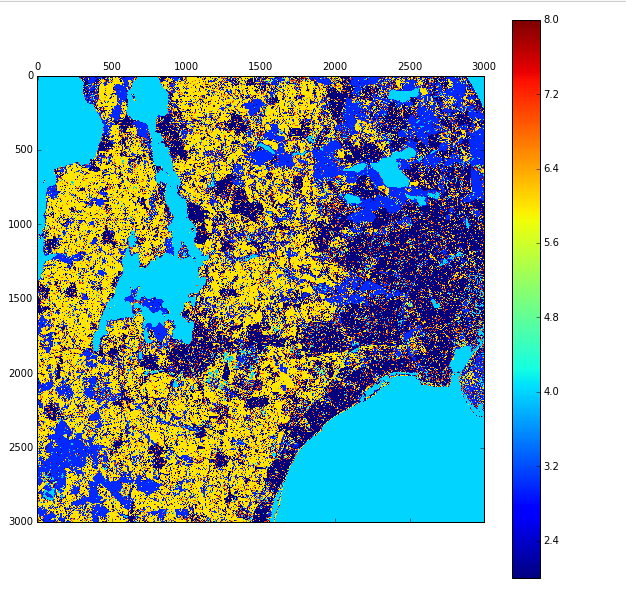
\includegraphics[width=10cm]{trees_pred.png}


\subsection{Runtime}
As stated on SKlearn's documentation(http://scikit-learn.org/stable/modules/tree.html), the construction time of a DecisionTree is $O(N_{samples} N_{features}\log(N_{samples}))$ and the query time is $O(\log(N_{samples}))$. We train 100 of them , therefore the time would be: $O(100 \cdot 10000 \cdot N_{features}\log(10000) =O(13.3\cdot10^6 N_{features})$


\subsection{Detecting Rare Instances}
The decision tree is a perfect choice for detecting rare instances in this specific case. Because all the other labels are 0, the gini index with the other parameters used in this model will attempt to find the best splits, and will create them where the space can be partitioned into 2 different labels. However, the problem here comes from the way we sample. 

We sample 10000 out of $10^9 = 1/10^5$ . We do this 100 times, so the class frequency in the sample is $1/10^3$. Therefore, there should be at least 1000 class 1 samples so that there would be on average 1 per tree. We only have 19, so the answer is we cannot detect the anomaly.